\documentclass[tikz, margin=3.14mm]{standalone}

\usepackage{tikz}
\usepackage{pgfplots}
\pgfplotsset{compat=1.18}

\pgfdeclarelayer{background}% determine background layer
\pgfsetlayers{background,main}% order of layers

\begin{document}

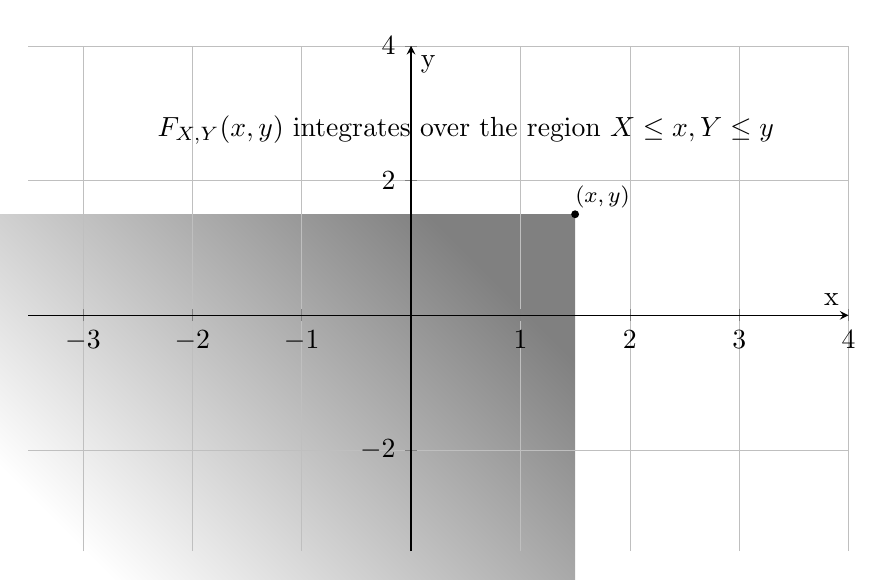
\begin{tikzpicture}
    \begin{axis}[
        xlabel = {x},
        ylabel = {y},
        % domain = -.4:4,
        xmax = 4,
        xmin = -3.5,
        ymin = -3.5,
        ymax = 4,
        samples = 100,
        title = {},
        axis lines = middle,
        width = 12cm,
        height = 8cm,
        clip = true,
    grid=both,
    grid style={line width=.1pt, draw=gray!10},
    major grid style={line width=.2pt,draw=gray!50},
    ]
    
    % \addplot[blue, thick, no markers] (-4,4) -- (0,0) -- (4, 0);
    \begin{pgfonlayer}{background}
    \shade[color = black!20, shading angle = -45] (-4,1.5) -- (1.5,1.5) -- (1.5,-4) -- (-4,-4) -- (-4, 1.5); 
    \end{pgfonlayer}
    
    \node [circle, inner sep = 0pt, minimum size = 1mm, fill = black] at (1.5, 1.5) {};
    
    \node at (0.5, 2.75) {$F_{X,Y}(x, y)$ integrates over the region $X \leq x, Y \leq y$};
    \node at (1.75, 1.75) {\footnotesize $(x, y)$};
    
    \end{axis}
\end{tikzpicture}

\end{document}